%% RNAAS comment on Zhao et al. (2026), J0008+0128
%% Compile with AASTeX v7.0.1 (aastex701.cls). No line numbers for RNAAS.
\documentclass{aastex701}

\newcommand{\msun}{\ensuremath{M_\odot}}
\newcommand{\rsun}{\ensuremath{R_\odot}}
\newcommand{\teff}{\ensuremath{T_{\rm eff}}}
\newcommand{\logg}{\ensuremath{\log g}}

\shorttitle{The companion of J0008+0128 need not be supermassive}
\shortauthors{Stevenson}

\begin{document}

\title{The dark companion of J0008+0128 need not be a supermassive neutron star}

\author[orcid=0000-0002-6100-537X]{Simon Stevenson}
\affiliation{Centre for Astrophysics and Supercomputing, Swinburne University of Technology, Hawthorn, VIC 3122, Australia}
\affiliation{ARC Centre of Excellence for Gravitational Wave Discovery (OzGrav), Australia}
\email[show]{spstevenson@swin.edu.au}

\begin{abstract}
\citet{Zhao2026} report J0008+0128 (Gaia DR3 2546630699873483008), a red giant in a 1218\,d orbit with a dark companion of mass $M_2=2.20^{+0.14}_{-0.13}$\,\msun, which they interpret as a likely supermassive neutron star. The mass function is precise, so the adopted giant mass, $M_1=1.67\pm0.15$\,\msun, sets the central value of the companion mass and the inclination sets its upper tail. The quoted uncertainties on both masses treat five estimates that share one radius and one inclination as independent, so they are too small. Two APOGEE DR17 value-added catalogues give a lighter giant: 1.22\,\msun\ from carbon and nitrogen abundances (DistMass) and 1.15\,\msun\ from isochrones (StarHorse). With $M_1=1.20\pm0.15$\,\msun, $M_2=1.85^{+0.27}_{-0.16}$\,\msun, with probabilities of 27\% and 8\% of exceeding 2.0 and 2.3\,\msun. That is comparable to Gaia NS1 and does not require a supermassive neutron star.
\end{abstract}

%% UAT keywords verified: Neutron stars (1108), Stellar masses (1614)
\keywords{\uat{Neutron stars}{1108} --- \uat{Stellar masses}{1614}}

\section{What sets the companion mass}

\citet{Zhao2026} fit radial velocities jointly with Gaia DR2 and DR3 astrometry and find period $P=1218\pm3$\,d, eccentricity $e=0.09\pm0.01$, velocity semi-amplitude $K_1=16.74\pm0.16$\,km\,s$^{-1}$ and inclination $i=73^\circ\pm11^\circ$, giving mass function $f(M)=0.587\pm0.017$\,\msun. At $i=73^\circ$, $M_2$ rises by about 0.6\,\msun\ for every 1\,\msun\ added to $M_1$ (Figure~\ref{fig:m1m2}), so the 0.5\,\msun\ spread of giant-mass estimates below moves $M_2$ by about 0.3\,\msun. Across $62$--$84^\circ$ the inclination changes $M_2$ by $+0.26/{-0.12}$\,\msun\ at $M_1=1.2$\,\msun. \citet{Zhao2026} adopt $M_1=1.67\pm0.15$\,\msun, a Bayesian combination of five values of $gR^2/G$ that use \logg\ from different pipelines and $R=5.39$\,\rsun\ from a spectral energy distribution fit at 1465\,pc, and combine the five companion masses in the same way to obtain $M_2=2.20^{+0.14}_{-0.13}$\,\msun.

Both values match the inverse-variance weighted means of the five inputs, which assumes the inputs are independent. They are not: all five giant masses share one radius, and all five companion masses share one inclination, whose uncertainty cannot average down. Propagating $M_1=1.67\pm0.15$\,\msun\ and $i=73^\circ\pm11^\circ$ directly gives $M_2=2.15^{+0.30}_{-0.16}$\,\msun, with a 28\% chance of exceeding 2.3\,\msun.

\begin{figure}[ht!]
\centering
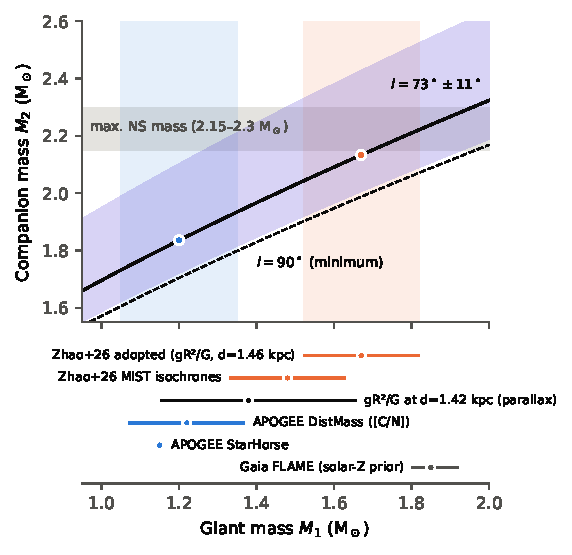
\includegraphics[width=0.56\textwidth]{fig_m1m2.pdf}
\caption{Top: companion mass against giant mass for $f(M)=0.587$\,\msun\ at $i=73^\circ$ (solid), $62$--$84^\circ$ (violet band) and $90^\circ$ (dashed); the grey band is the maximum neutron star mass. Columns mark $M_1=1.20\pm0.15$\,\msun\ (blue, this note) and $1.67\pm0.15$\,\msun\ (orange, \citealt{Zhao2026}); points give $M_2$ at $i=73^\circ$. Bottom: individual giant-mass estimates; StarHorse has no error bar.\label{fig:m1m2}}
\end{figure}

\section{A lighter giant}

The APOGEE DR17 \citep{Abdurrouf2022} parameters are $\teff=4955$\,K, $\logg=3.144\pm0.024$, [M/H]$\,=-0.26$ and [C/N]$\,=-0.18$. DistMass \citep{StoneMartinez2024}, a neural network trained on asteroseismic masses, gives $M_1=1.22\pm0.15$\,\msun\ from these parameters without using a distance (the uncertainty is its stated 12\% scatter). StarHorse \citep{Queiroz2023}, which fits isochrones using the Gaia parallax, gives 1.15\,\msun\ at 1.32\,kpc. \citet{Zhao2026} obtain 1.45--1.52\,\msun\ by fitting MIST isochrones \citep{Dotter2016,Choi2016} to the APOGEE parameters, photometry and parallax; a 1.45\,\msun\ track reaches the APOGEE \logg\ at $\teff\approx5000$\,K, about 40\,K hotter than the corrected $\teff=4964\pm40$\,K in their Table S2. At 4964\,K the tracks give 1.29\,\msun\ from \logg\ alone and 1.30\,\msun\ on the HR diagram at 1.42\,kpc; at about 0.4\,\msun\ per 100\,K, these masses depend strongly on the temperature scale.

The $gR^2/G$ mass scales as $d^2$ at fixed \logg. With the APOGEE \logg\ it gives $M_1=1.48$\,\msun\ at 1465\,pc and 1.16--1.21\,\msun\ at the 1.30--1.32\,kpc preferred by DistMass and StarHorse. The corrected \logg\ values in the same table are 3.14--3.20 from APOGEE (DR17 and SDSS-V) and LAMOST medium-resolution spectra, but 3.27 and 3.30 from LAMOST low-resolution spectra, so their 1.67\,\msun\ requires both the larger distance and these higher \logg\ values. Their distance also omits the parallax zero point: 1464.6\,pc is exactly $1/\varpi$ for the Gaia DR3 \citep{GaiaDR3} parallax, and their fitted parallax offset is $0.00\pm0.03$\,mas. The \citet{Lindegren2021} correction for this star, $-0.023$\,mas, gives $1.416\pm0.060$\,kpc and $M_1=1.38\pm0.26$\,\msun.

Gaia DR3 FLAME gives $M_1=1.85$\,\msun\ from solar-metallicity tracks \citep{Creevey2023}, which bias the mass high for a giant at [M/H]$\,=-0.26$; its luminosity and radius imply $\teff\approx5060$\,K, at which MIST gives 1.70\,\msun\ with the APOGEE \logg. Its age of 1.46\,Gyr is also below the 1.5\,Gyr limit \citet{Fouesneau2023} recommend for giant masses, and its radius ($5.07$\,\rsun) with the APOGEE \logg\ gives 1.31\,\msun.

Taking $M_1=1.20\pm0.15$\,\msun\ (between the DistMass and StarHorse values), $i=73^\circ\pm11^\circ$ and $f(M)=0.587\pm0.017$\,\msun\ with Gaussian errors, a Monte Carlo gives $M_2=1.85^{+0.27}_{-0.16}$\,\msun, at the low end of the 1.8--2.8\,\msun\ range \citet{Zhao2026} quote as spanning all estimates. $P(M_2>2.0\,\msun)=0.27$ and $P(M_2>2.3\,\msun)=0.08$, where 2.0\,\msun\ is their threshold for a supermassive neutron star and 2.3\,\msun\ the top of the maximum neutron star masses they quote; almost all draws above 2.3\,\msun\ have $i<62^\circ$. The conclusion does not rest on the lowest giant mass: $M_1=1.30\pm0.20$\,\msun\ (the MIST track masses, with a wider uncertainty) gives $P(M_2>2.3\,\msun)=0.11$, and the parallax-based $M_1=1.38\pm0.26$\,\msun\ gives 0.15, compared with 0.28 for $M_1=1.67\pm0.15$\,\msun. These $M_2$ values use no neutron star population prior; applying one would likely lower them further \citep{Farr2020}.

DistMass and StarHorse both use these APOGEE parameters, so they are not fully independent, but neither uses the LAMOST \logg\ values or the joint-fit distance. Material accreted from the neutron star's progenitor would probably be nitrogen-rich, biasing the [C/N] mass upward (+0.05\,dex in nitrogen adds about 0.05\,\msun\ in the \citealt{Martig2016} fit), so the giant could be lighter still. The DistMass spectroscopic distance ($1.30\pm0.09$\,kpc) agrees with StarHorse and is only 1--1.5$\sigma$ from 1.42--1.46\,kpc, so I give more weight to the distance-independent [C/N] mass. The parallax distance still gives $M_2=1.95$\,\msun\ (zero-point corrected) or 2.02\,\msun\ (uncorrected) at $i=73^\circ$, below the maximum neutron star mass.

Public DR17 estimates favour $M_1\approx1.2$\,\msun\ and $M_2\approx1.9$\,\msun: a heavy neutron star in a wide, nearly circular orbit, like Gaia NS1 \citep{ElBadry2024}, rather than a supermassive one. Epoch astrometry from the imminent Gaia DR4, fitting the orbit and parallax together, should fix the inclination and distance, and hence the giant's radius and mass.

\begin{acknowledgments}
This research was funded in part by the Australian Research Council Centre of Excellence for Gravitational Wave Discovery (OzGrav; CE230100016).
\end{acknowledgments}

\begin{contribution}
AI disclosure: I used Claude (Anthropic; Claude Opus 5.5) to help retrieve and check catalogue values, run the calculations, write the figure code and draft the text; I verified all inputs and results.
\end{contribution}

%% Zenodo concept DOI (all versions)
The code and input values are available at \url{https://github.com/SimonStevenson/j0008-rnaas} (archived on Zenodo: \doi{10.5281/zenodo.24293381}).

\facilities{Gaia, Sloan}

\software{NumPy, SciPy, Matplotlib, gaiadr3-zeropoint}

%% All references checked against ADS or publisher records
\begin{thebibliography}{}
\bibitem[Abdurro'uf et al.(2022)]{Abdurrouf2022} Abdurro'uf, et al. 2022, ApJS, 259, 35
\bibitem[Choi et al.(2016)]{Choi2016} Choi, J., et al. 2016, ApJ, 823, 102
\bibitem[Creevey et al.(2023)]{Creevey2023} Creevey, O.~L., et al. 2023, A\&A, 674, A26
\bibitem[Dotter(2016)]{Dotter2016} Dotter, A. 2016, ApJS, 222, 8
\bibitem[El-Badry et al.(2024)]{ElBadry2024} El-Badry, K., et al. 2024, OJAp, 7, 27
\bibitem[Farr \& Chatziioannou(2020)]{Farr2020} Farr, W.~M., \& Chatziioannou, K. 2020, RNAAS, 4, 65
\bibitem[Fouesneau et al.(2023)]{Fouesneau2023} Fouesneau, M., et al. 2023, A\&A, 674, A28
\bibitem[Gaia Collaboration et al.(2023)]{GaiaDR3} Gaia Collaboration, Vallenari, A., et al. 2023, A\&A, 674, A1
\bibitem[Lindegren et al.(2021)]{Lindegren2021} Lindegren, L., et al. 2021, A\&A, 649, A4
\bibitem[Martig et al.(2016)]{Martig2016} Martig, M., et al. 2016, MNRAS, 456, 3655
\bibitem[Queiroz et al.(2023)]{Queiroz2023} Queiroz, A.~B.~A., et al. 2023, A\&A, 673, A155
\bibitem[Stone-Martinez et al.(2024)]{StoneMartinez2024} Stone-Martinez, A., et al. 2024, AJ, 167, 73
\bibitem[Zhao et al.(2026)]{Zhao2026} Zhao, X., et al. 2026, SciA, 12, eaeg3307
\end{thebibliography}

\end{document}
